\chapter{Nulla-ismeretű protokollok azonosításra}

A nulla-ismeretű protokollok egyik elterjedt alkalmazása a felhasználók azonosítása, autentikálása. Ebben a fejezetben ilyen protokollokat fogunk áttekinteni.

\section*{A Schnorr azonosító protokoll}

Ezt megelőzően is léteztek már nulla-ismeretű protokollok, mint Fiat-Shamir \cite{FiatShamir} és annak továbbfejlesztései (FFS \cite{FeigeFiatShamir} és GQ protokollok \cite{GuillouQuisquater}), amelyek biztonsságosságukat a faktorizációs probléma nehézségéből nyerik. 

A Schnorr protokoll \cite{Schnorr}, ezzel ellentétben biztonságát a diszkrét logaritmus problémából nyeri. Manapság az elliptikus görbe kriptográfia egyre nagyobb teret nyer, köszönhetően a kisebb kulcsméretnek, vele együtt pedig növekszik az elliptikus görbe diszkrét logaritmus probléma. Ezért úgy érzem előnyösebb Schnorr protokollját áttekinteni, mint az őt megelőző faktorizáción alapuló protokollokat.

\subsection*{A diszkrét logaritmus probléma}\cite{BerczesPetho}

\begin{definition}
    Legyen $m$ egy pozitív egész szám. Egy $g$ egész számot primitív gyöknek nevezünk modulo $m$ ha minden $b \in \{1,2,...,m-1\}$ szám esetén, melyre $(b,m) = 1$ létezik olyan $k$ pozitív egész szám, melyre $g^k \equiv b \pmod{m}$.
\end{definition}

\begin{theorem}
    Akkor, és csakis akkor létezik primitív gyök modulo $m$, ha $m = 2$, $m = 4$, $m = p^k$ vagy $m = 2p^k$, ahol $p$ valamely pozitív szám.
\end{theorem}

\begin{definition}
    Legyen $p$ egy pozitív prímszám, $b$ egy egész szám, melyre $(b, p) = 1$, és legyen $g$ egy primitív gyök modulo $p$. Azt a legkisebb pozitív egész $k$ számot, melyre teljesül, hogy $g^k \equiv b \pmod{p})$ a $b$ szám $g$ alapú diszkrét logaritmusának nevezzük modulo $p$.
\end{definition}

Miközben a modulo $p$ történő hatványozás nagy $p$ értékek esetén is gyorsan kiszámítható, addig ennek megfordítása, a diszkrét logaritmus kiszámítása nagyon időigényes feladat.

\subsection*{A Schnorr azonosító protokoll algoritmusa}

A protokol a rendszer paraméterek inicializáló lépésével indul.

\begin{algorithm}[H]
    \floatname{algorithm}{Algoritmus}
    \caption{Rendszer inicializáció}
    \label{algorithm:systemInit}
    \begin{algorithmic}
        \Procedure{sys\_init}{$t$} \Comment $2^{-t}$ a rendszerben a helyes tippelés valószínűsége
        \State $p$ prím inicializálása
        \State $q$ prím inicializálása \Comment $q | p-1$
        \State $\alpha$ elem kiválasztása \Comment $\alpha \in \mathbb{Z}_{p}$ és rendje $q$
        \EndProcedure
    \end{algorithmic}
\end{algorithm}

\begin{algorithm}[H]
    \floatname{algorithm}{Algoritmus}
    \caption{Felhasználói paraméterek generálása}
    \label{algorithm:userInit}
    \begin{algorithmic}
        \Procedure{user\_init}{$I_{A}$} \Comment $I_{A}$ a felhasználó egyedi azonosítója
        \State $s$ privát kulcs generálása \Comment ez egy random szám az $\{1,2,...,q\}$ halmazból
        \State $v = \alpha^{-s} \pmod{p}$ publikus kulcs kiszámítása
        \State $\alpha$ elem kiválasztása \Comment $\alpha \in \mathbb{Z}_{p}$ és rendje $q$
        \State A rendszerrel aláíratja az $(I_{A}, v)$ párost, ezzel előáll $sign_{A}$
        \EndProcedure
    \end{algorithmic}
\end{algorithm}

Ezt követően az azonosító protokoll-t mutatja a \ref{Figure::SchnorrProt} ábra:

\begin{figure}[H]
    \centering
    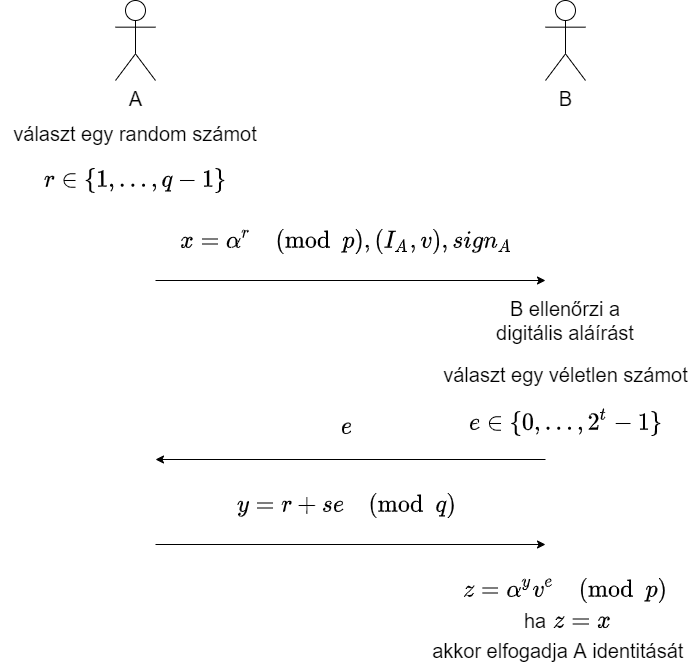
\includegraphics[width=0.6\textwidth]{Schnorr-protokoll.png}
    \caption{Schnorr azonosító protokoll.}
    \label{Figure::SchnorrProt}
\end{figure}

\subsection*{A Schnorr azonosító protokoll biztonságossága}

\begin{itemize}
    \item Biztonság: A biztonságosság egyik fő szereplője a $t$, ezt olyan módon kell megválasztani, hogy $2^{-t}$ kellően kicsi legyen, hiszen ez a valószínűsége a helyes tippelésnek a választott $e$ értékre. A másik fontos pontja a protokollnak a megfelelő méretű $q$ választása, mert ez felelős a diszkrét logaritmus probléma nehézségéért.
    \item Megalapozottság: A protokollt áttekintve, belátható, hogy $s$ ismerete nélkül nem lehetséges senki számára, hogy $A$-nak adja ki magát, mert ezen információ ismeretében képes csak sikeresen végigjátszani a folyamatot.
    \item Nulla-ismeret: A protokoll csak akkor teljesíti a nulla-ismeret tulajdonságot, ha a hitelesítő fél becsületesen jár el. Ez azt jelenti, hogy az $e$ értéket valóban random módon választja ki és nem a kapott $x$ értékétől függően. Ha $x$ értéke alapján választ egy számára megfelelő $e$-t, akkor képes információt kinyerni a felhasználó a bizonyító fél titkával kapcsolatban.
\end{itemize}

\begin{minipage}{\textwidth}
Ezen felül rendkívül fontos követelménye ennek a protokollnak, hogy egy interaktív folyamat során ne használjuk kétszer ugyanazt a random $r$ értéket, hiszen ha kétszer használnánk egyszerűen kiszámíthatóvá vális az $s$ titkunk a következő módon:

$(y_1 - y_2) / (e_1 - e_2) \pmod{q}$ \\
$= (r + se_1) - (r + se_2) / (e_1 - e_2) \pmod{q}$ \\
$= s(e_1 - e_2) / (e_1 - e_2) \pmod{q}$ \\
$= s$
\end{minipage}

\section*{M-Pin protokoll}

Az M-Pin protokoll \cite{MPin} egy rendkívül modern elgondolása az autentikációnak, ami a jelenlegi felhasználónév és jelszó alapú rendszerek egy működőképes alternatívája. Ahogy korábban is említettem a jelszavas rendszerek nagy hátránya, hogy a szervereken létezik egy adatbázis amiben a felhasználói jelszavak tárolásra kerülnek többnyire hash-elt változatban (azonban még előfordulnak olyan esetek is, amikor a tényleges jelszót tárolják). Ezeket az adatbázisokat gyakran feltörik és ellopják.

Az M-Pin célja az, hogy a regisztrált felhasználóknak osszunk ki egy nagy kriptográfiai titkot, amelyet felhasználva nulla-ismeretű bizonyítékkal képes igazolni kilétét. Így nincs szükség arra, hogy bármilyen felhasználói titkot tároljon a szolgáltató a szerverein.

Mielőtt áttekintenénk, hogyan is működik ez az eljárás, fontos ismernünk az elliptikus görbék és a párosítás alapjait.

\subsection*{Elliptikus görbe kriptográfia}

\subsection*{Párosítás-alapú kriptográfia}

\subsection*{Az M-Pin protokoll algoritmusa}